\chapter{Enlace cristalino}

En este capítulo se estudian los distintos mecanismos de \textit{cohesión} de los cristales. La \textit{distribución electrónica} alrededor de los núcleos caracteriza, a nivel microscópico, el tipo de enlace cristalino: \textit{covalente, metálico, molecular, iónico} y \textit{de hidrógeno}. La \textit{energía de cohesión} (aquella que se debe suministrar al cristal para separarlo en sus constituyentes) varía para los elementos cristalinos desde 0.02 eV/átomo en el Ne hasta 8.9 en el W.

\section{Clasificación de los sólidos}

El cálculo de la energía de cohesión requiere el conocimiento de los estados electrónicos en el cristal. Las funciones de onda electrónicas de los electrones de valencia de los átomos libres cambian (y en consecuencia la distribución de carga) cuando los átomos se unen formando el cristal. En función de cuánto cambian estos estados electrónicos, los sólidos suelen clasificarse en cuatro tipos fundamentales, con distribuciones electrónicas según muestra la figura \ref{Fig:03-01}:

\begin{itemize}
    \item \textbf{Moleculares}: con cambio mínimo.
    \item \textbf{Iónicos} en los que hay trasferencia de carga.
    \item \textbf{Covalentes} en los que la distribución de carga es direccional y localizada.
    \item \textbf{Metálicos} con carga electrónica extendida a todo el cristal.
\end{itemize}

\begin{figure}[h!] \centering
    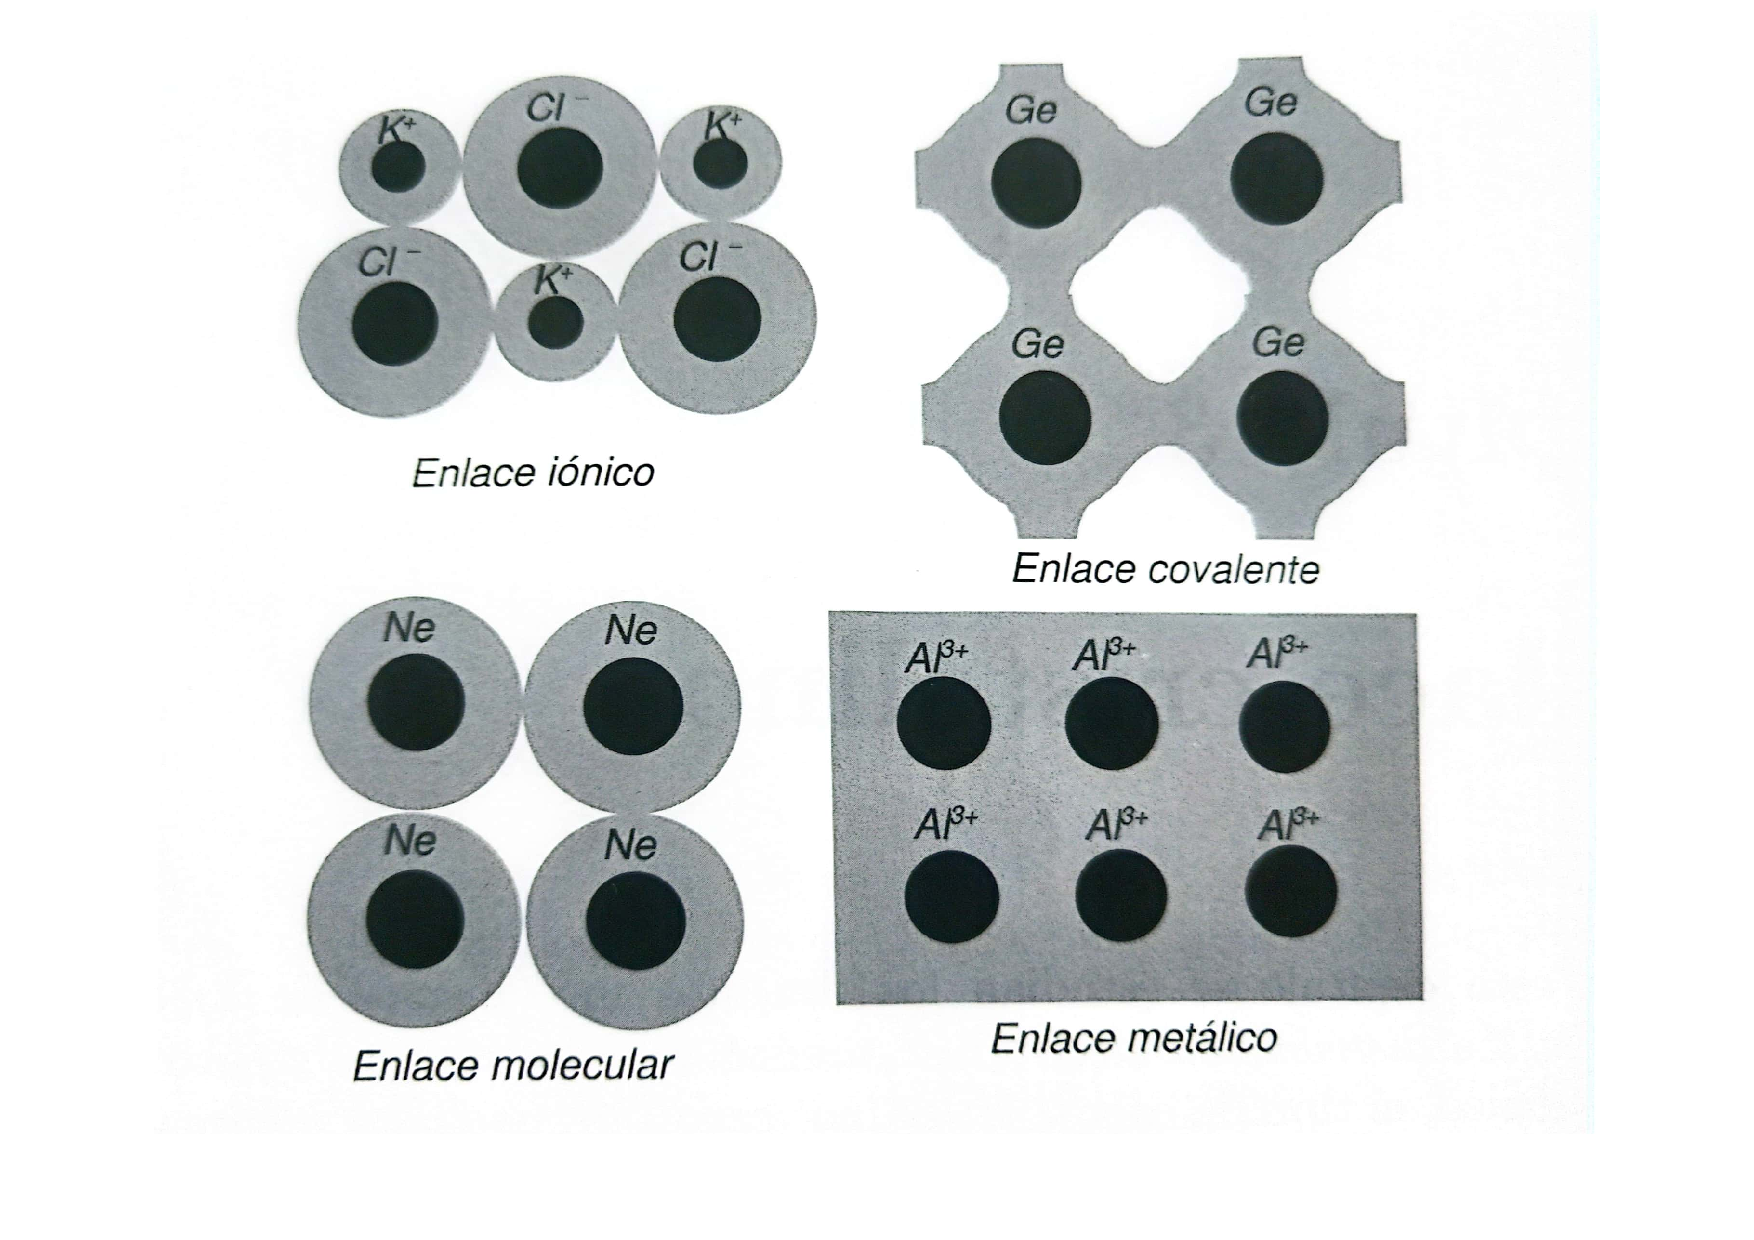
\includegraphics[scale=0.5]{Cuerpo/Ch_03/Fotos libro 1.pdf}
    \caption{Esquema de la distribución electrónica en los tipos de sólidos básicos}
    \label{Fig:03-01}
\end{figure}    

\section{Cristales moleculares}

Son aquellos en que los nudos están ocupados por moléculas en las que los \textit{enlaces intermoleculares son débiles} (al menos respecto los intramoleculares). Ejemplo de estos son los gases inertes y gases orgánicos (metano...). Los átomos de gases inertes tienen las capas electrónicas cerradas con simetría esférica. La baja energía de ionización ($\sim 1 \%$) sugiere que la distribución de carga no se distorsiona apreciablemente. 


\subsection{Interacción de \textit{van der Waals-London}}


La deformación atómica más sencilla que conduce a una interacción no nula entre átomos es el desplazamiento de la nube electrónica (\textit{rígida}) de manera que aparezca un momento dipolar. El modelo simple que muestra en la figura \ref{Fig:03-02} en el que se supone $x_1,x_2\ll R$, permite dar cuenta de la existencia de una interacción atractiva entre átomos o moléculas neutros. 

La energía de los dos osciladores sin interacción ($R\rightarrow \infty$) esférica

\begin{equation}
    H_0 = \frac{p_1^2}{2M} + \frac{1}{2} Cx_1^2 + \frac{p_2^2}{2M} + \frac{1}{2} Cx_2^2
\end{equation}

\begin{figure}[h!] \centering
    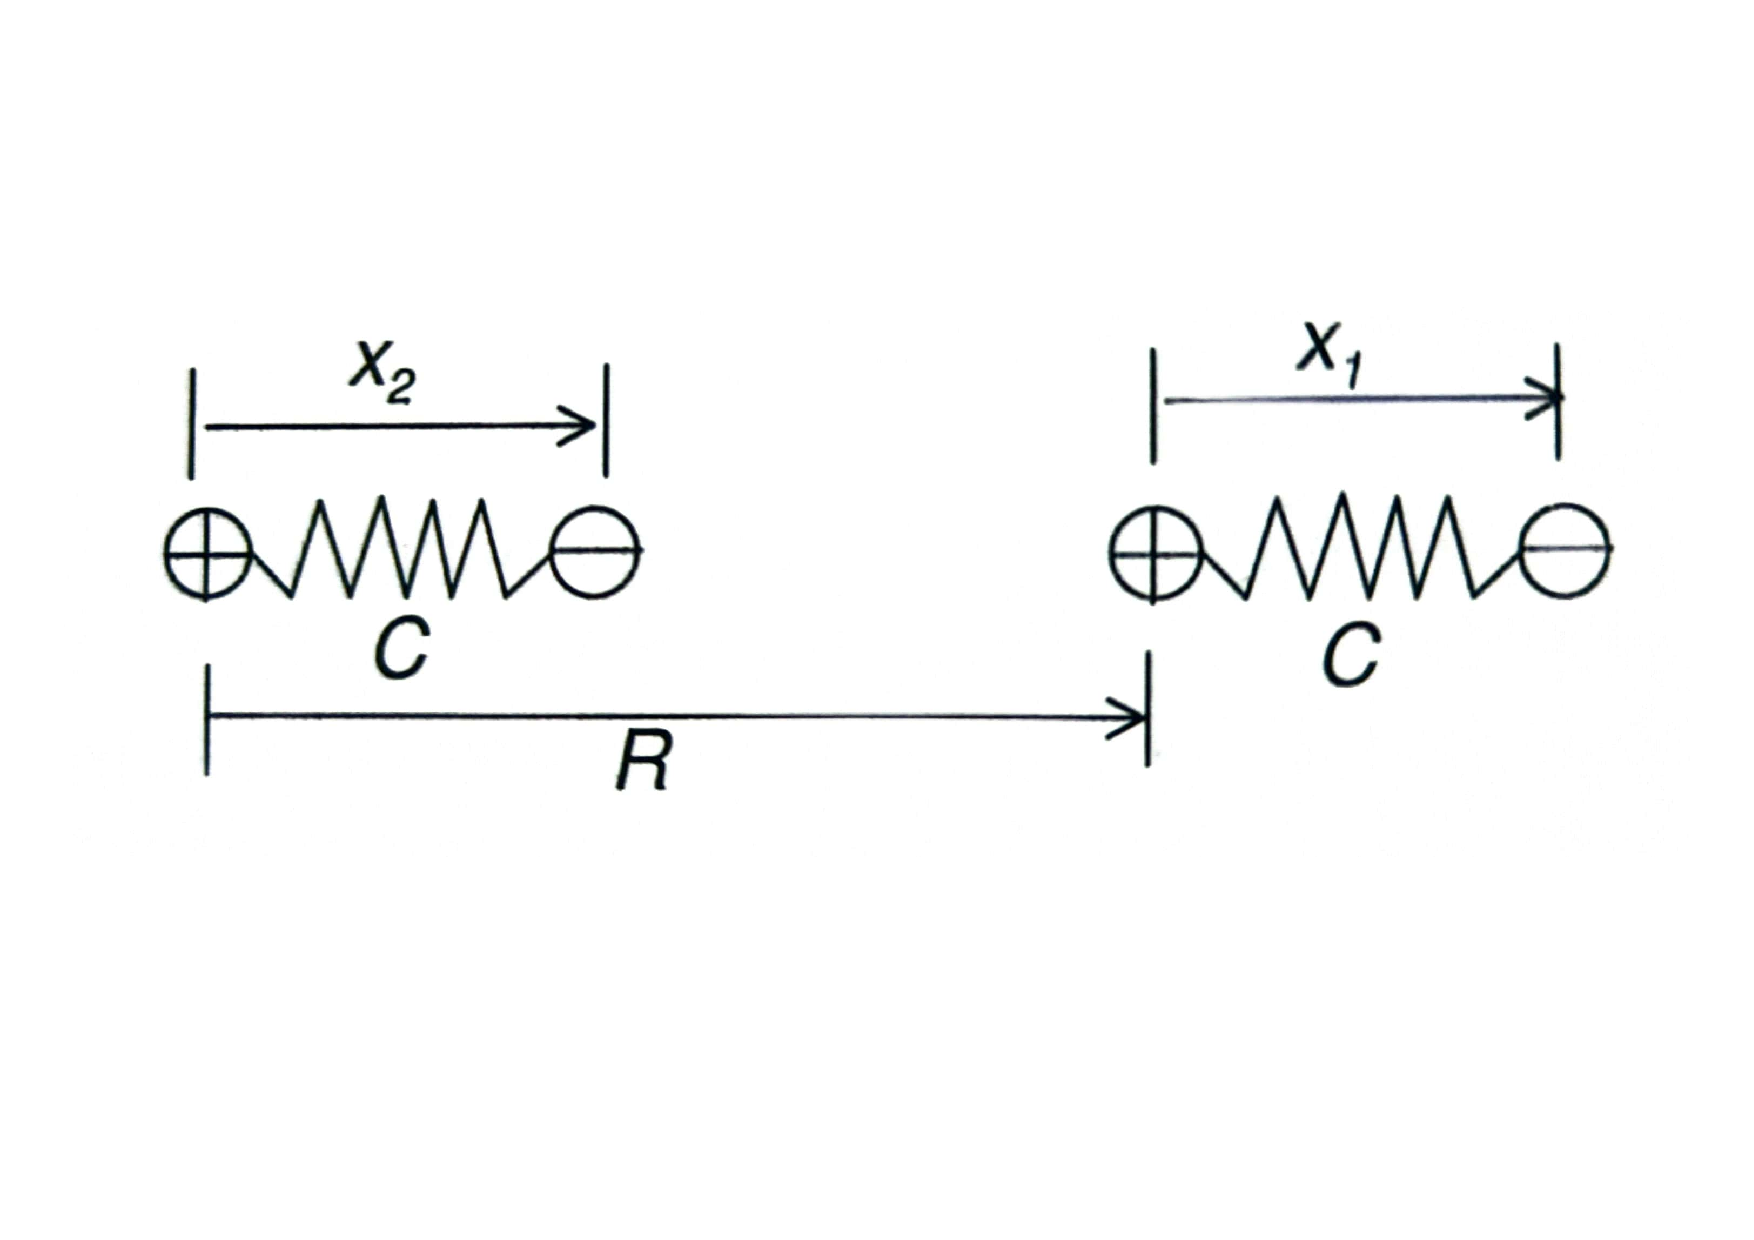
\includegraphics[scale=0.5]{Cuerpo/Ch_03/Fotos libro 2.pdf}
    \caption{Posiciones relativas de los osciladores.}
    \label{Fig:03-02}
\end{figure}    

donde $C=M\omega_0^2$ siendo $\omega_0$ la frecuencia propia de vibración de la carga (rígida) negativa de los átomos y $M$ su masa. Por su parte, la energía de interacción de Coulomb se expresa por 

\begin{equation}
    H_i = \frac{q^2}{R} + \frac{q^2}{R+x_1-x_2} - + \frac{q^2}{R+x_1} - + \frac{q^2}{R-x_2} \approx - \frac{2q^2x_1x_2}{R^3}
\end{equation}
donde $q^2=e^2$ en unidades cgs o $q^2 = e^2 / 4\pi \epsilon_0$ en mks. El hamiltoniano total $H=H_0+H_i$ se puede diagonalizar para obtener sus valores propios, introduciendo las llamadas {\it variables normales}

\begin{align}
    x_s \equiv \frac{1}{\sqrt{2}} (x_1 + x_2)  \tquad  & x_a \equiv \frac{1}{\sqrt{2}} (x_1-x_2) \\
    p_s \equiv \frac{1}{\sqrt{2}} (p_1 + p_2) \tquad & p_a \equiv \frac{1}{\sqrt{2}} (p_1-p_2) 
\end{align}
de modo que 

\begin{equation}
    H = \ccorchetes{\frac{p_s^2}{2M}+ \frac{1}{2} \parentesis{C- \frac{2q^2}{R^3}}x_s^2} + \ccorchetes{\frac{p_a^2}{2M}+ \frac{1}{2} \parentesis{C+ \frac{2q^2}{R^3}}x_a^2} 
\end{equation}
Formalmente el problema se reduce al de dos \textit{osciladores} independientes, de frecuencias propias:

\begin{equation}
\omega_s^2 = \omega_0^2 - \frac{2q^2}{MR^3} \quad \omega_a^2 = \omega_0^2 + \frac{2q^2}{MR^3}
\end{equation}
El cambio en la energía (por oscilador) debido al acoplamiento será $\Delta E = \frac{1}{2} (\hbar \omega_s + \hbar \omega_a - 2 \hbar \omega_0$), qe en la aproximación  $ \frac{2q^2}{MR^3} \ll \omega_0^2$ es

\begin{equation}
\Delta E \approx - \frac{1}{2} \hbar \omega_0 \parentesis{\frac{q^2}{CR^3}}^2 \propto -C^{-3/2}  R^{-6} \label{Ec:03-02-07}
\end{equation}
La dependencia (\ref{Ec:03-02-07}) coincide con la clásica \textit{dipolo-dipolo inducido}. Observar sin embargo que la interacción es un efecto cuántico en cuanto que $\Delta E \rightarrow 0$ si $\hbar \rightarrow 0$. 

\textbf{Interacción repulsiva}. Además de la \textit{repulsión electroestática} entre las nubes electrónicas, el \textit{Principio de Pauli} impide que átomos con capas llenas puedan solaparse a menos que haya promoción parcial de los electrones a estados energéticos más altos desocupados (lo cual implicaría un costo de energía). Es de esperar entonces que la interacción repulsiva sea de corto alcance y, en efecto, los datos experimentales de los gases inertes pueden ajustarse bien por un potencial \textit{semiempírico} con dependencia de la separación entre átomos según $R^{-12}$.

\subsection{Interacción de Lennard-Jones}


El potencial de interacción por par de átomos $i$ y $j$ (a distancia $r_{ij}$) resultante (contribución atractiva más repulsiva) puede escribirse Coulomb

\begin{equation}
    U (r_{ij}) = 4 \epsilon \ccorchetes{\parentesis{\frac{\sigma}{r_{ij}}}^{12}-\parentesis{\frac{\sigma}{r_{ij}}}^6}
\end{equation}
Esta ecuación describe la llamada \textbf{intearcción de Lennard-Jones} o  \textbf{interacción 6-12}. Un modelo parecido a este es el \textit{modelo de las esferas duras}, en el que $U(r_{ij})$ definida a cachos de tal modo que para $r<R$ (siendo $R$ el radio del átomo/molécula/ión) tendremos que $U = \infty$. Sin embargo esta función experimental, describe mucho mejor el comportamiento de los sólidos. Los parámetros $\epsilon$ y $\sigma$ pueden determinarse a partir de medidas de viscosidad y coeficientes de virial en la fase gaseosa. El potencial total sobre un átomo $i$ cualquiera esférica

\begin{equation}
    U_i = \sum_{j\neq i}^N U(r_{ij}) = 4 \epsilon \ccorchetes{B \parentesis{\frac{\sigma}{R}}^{12}-A\parentesis{\frac{\sigma}{R}}^6} \quad \text{con} \ B = \sum_{i\neq j}^N p_{ij}^{-12} \quad A = \sum_{i\neq j}^N p_{ij}^{-6} 
\end{equation}
siendo $R$ la distancia entre vecinos más proximos y $p_{ij}=r_{ij}/R$. Las sumas $A$ y $B$ dependen de la estructura cristalina. En el cuadro \ref{Tab:03-01} (izquierda) se dan sus valores para algunas de las más comunes. Para calcular estos parámetros podemos usar aproximaciones a primeros vecinos/segundos vecinos, o usar métodos computacionales. 

\begin{figure}[h!] \centering
    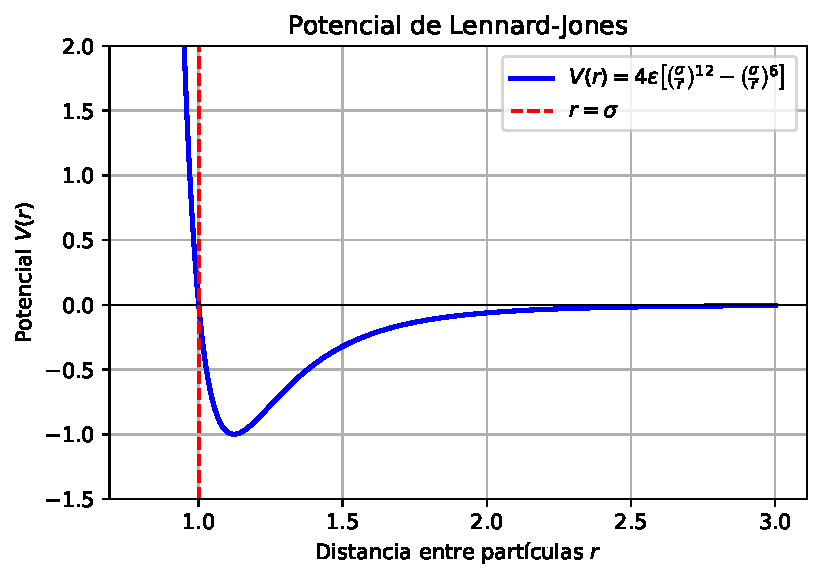
\includegraphics[scale=1.05]{Cuerpo/Ch_03/Lennard-jones.pdf}
    \caption{Potencial de Lennard-jones para variables reducidas ($\epsilon,\sigma = 1$)}
    \label{Fig:03-03}
\end{figure}    

El potencial total del cristal resulta

\begin{equation}
    U = \frac{1}{2} \sum_i^N U_i = 2 \epsilon N \ccorchetes{B\parentesis{\frac{\sigma}{R}}^{12}-A\parentesis{\frac{\sigma}{R}}^6} \label{Ec:03-02-10}
\end{equation}
A partir de la ecuación \ref{Ec:03-02-10} se puede calcular la distancia de equilibrio $R_0$ por la condición $(\D U / \D R)_{R_0} =0$ obteniéndose $R_0 / \sigma = (2B/A)^{1/6}$ (1.09 para una estructura \textit{fcc}). Los valores experimentales para algunos gases nobles (\textit{fcc}) son los mostrados en el cuadro  \ref{Tab:03-01} (derecha). La pequeña desviación de los átomos más ligeros se debe a \textit{efectos cuánticos del punto cero}. Esto se entiende por el espacio de confinamiento del átomo en el cristal, la energía cinética será $p^2/2m= (h/\lambda)^2/2m$: inversamente proporcional a la masa. 

En cuanto a la energía de cohesión (en equilibrio) a temperatura cero se puede obtener sin más que sustituir en \ref{Ec:03-02-10} $R=R_0$ resultando

\begin{equation}
U_0 \equiv (R_0) = - N\epsilon (A^2/2B)
\end{equation}
La estructura con menor $U_0$ es la \textit{fcc} ($-8.6 N\epsilon$), que es la que tienen todos los cristales de gases nobles. Las correciones mecanocuánticas a $U_0$ alcanzan casi un 30\% en el Ne y hasta un  4\% en el Xe. Las diferencias entre energías son muy pequeñas entre la \fcc y a \hcp, tal y como podemos ver en la siguiente tabla (tabla \ref{Tab:03-01}). La razón de esto es que ambas estructuras, tal y como hemos visto en el capítulo \ref{Ch:01} son las estructuras compactas por antonomasia, por lo que las diferencias energéticas entre ambas serán diferentes. Que un sólido adopte una u otra dependerá de la variación del potencial de Lennard-jones o de las posibles impurezas.

\begin{table}[h!] \centering
\begin{tabular}{ccccccccc}
Estructura & B & A & & Elemento & Ne & Ar & Kr & Xe \\ \cline{1-3} \cline{5-9} 
\fcc & 12.122 & 14.454 & \quad & $R_0/\sigma$ & 1.14 & 1.11 &1.10 & 1.09 \\
\hcp & 12.132 & 14.455 & & $-U/N\epsilon$ & 5.59 & 8.24 & 8.61 & 8.62 \\
\bcc & 9.114 & 12.253 & & $-U_0 (\unit{\eV}/\text{at.})$ & 0.02 & 0.08 & 0.12 & 0.17\end{tabular}
\caption{A la izquierda los parámetros A y B para las estrucutras indicadas. A la derecha valores experimentales para los cristales de gases nobles con estrucutra \fcc.}
\label{Tab:03-01}
\end{table}

% hablar de criogenia, superfluidos, 

\section{Cristales iónicos}
Son los formados por iones positivos y negativos. En este tipo de cristales uno de los iones forma una estructura mientras que el otro ion se va metiendo en los huecos. El enlace iónico es fuerte (6-12 eV/ion) y es el resultado de la interacción electroestática \textit{directa} de iones con \textit{capas electrónicas completas}, como por ejemplo el $\Namas$ ($1s^22s^2 2p^6)$ y $\Clmenos$ ($1s^22s^2 2p^6 3s^2 3p^6$).

\textbf{Constante de Madelung.} Aparece al calcular la energía (potencial) de cohesión de un cristal iónico admitiendo una energía potencial por pares de forma 

\begin{equation}
    U_{ij} = \frac{\pm q^2}{r_{ij}} + \frac{B}{r_{ij}^n} \label{Ec:03-03-01}
\end{equation} 
donde $B$ y $n$ ($n\gg 1$) son desconocidos ($q^2 = e^2$ en unidades cgs o $q^2=e^2 / 4 \pi \epsilon_0$ en mks). Otra aproximación válida sería utilizar una intersección repulsiva de la forma $\lambda e^{-r_{ij}/\rho}$. Análogamente a las sumas en \ref{Ec:03-02-10}, al sumar \ref{Ec:03-03-01} para todos los pares (N átomos) se tiene 

\begin{equation}
    U = \frac{N}{2} \parentesis{\frac{BA_n}{R^n}-\frac{\alpha q^2}{R}}
\end{equation}
con 

\begin{equation}
    A_n = \sum_{i\neq j} p_{ij}^{-n} \tquad \alpha = \sum_{j \neq i} \pm p_{ij}^{-1} \quad p_{ij} = \frac{r_{ij}}{R}
\end{equation}
tal que a $\alpha$ se conoce como \textbf{constante de Madelung} y su valor depende de la estructura (cuadro \ref{Tab:03-02}).

\begin{table}[h!] \centering
    \begin{tabular}{c|ccc}
        Estrucura & ClNa & ClCs & ZnS cúbica \\ \hline
        $\alpha$ & 1.748 & 1.763 & 1.638 
    \end{tabular}
    \caption{Constante de Madelung para algunas estructuras muy comunes.}
    \label{Tab:03-02}
\end{table}

La separación de equilibrio $R_0$ se calcula a partir  de la condición $(\partial U / \partial R)_{R_0} = 0 \Rightarrow R_0 = (nBA_n/\alpha q^2)^{1/(n-1)}$, a la cual

\begin{equation}
U(R_0) = - \frac{N}{2} \frac{\alpha q^2}{R_0} \parentesis{1-\frac{1}{n}} \label{Ec:03-03-04}
\end{equation}
El exponente $n$ puede relacionarse con el coeficiente de compresibilidad $K\equiv - V^{-1}(\partial V / \partial P)_{R_0}$ (donde $P$ es la presión y $V$ el volumen) según $n=1+18R_0^4 / Kq^2 \alpha$. Como ejemplo para el NaCl (\fcc), a partir del valor experimental $K=3.3\times 10^{-12} \unit{\cm}^2 / \text{dyna}$ y $\alpha = 1.75$ se obtiene $n=9.4$. También para el NaCl se obtiene que $\rho=0.3 \ \unit{\angstrom}$ admitiendo una forma exponencial para la interacción repulsiva, de modo que resulta ser ésta de muy corto alcance.

% Revisar y ampliar

Las energías de cohesión de cristales iónicos típicos como los haluros alcalinos se predicen según ecuación \ref{Ec:03-03-04}, con una precisión mejor que el 10\%. El término $-N\alpha q^2 / 2 R_0$ representa prácticamente el 90\% de $U(R_0)$. En el cuadro \ref{Tab:03-03} se dan estos valores para  algunos \textit{haluros alcalinos}.

\begin{table}[h!] \centering
    \begin{tabular}{c|ccccc}
        & Li & Na & K & Rb & Cs \\ \hline
        F & 10.5 & 9.31 & 8.25 & 7.86 & 7.50 \\
          & \textbf{12.6} & \textbf{10.9} & \textbf{9.44} & \textbf{8.94} & \textbf{8.38} \\ \hline
        Cl & 8.63  & 7.94 & 7.19 & 6.94 & \\
           & \textbf{9.82} & \textbf{8.94} & \textbf{8.00} & \textbf{7.69} & \\ \hline  
        Br & 8.25 & 7.56 & 6.86 & 6.63 & \\
           & \textbf{9.19} & \textbf{8.44} & \textbf{7.63} & \textbf{7.38} & \\ \hline
        I & 7.69 & 7.06 & 6.50 & 6.31 & \\
        & \textbf{8.38} & \textbf{7.75} & \textbf{7.13} & \textbf{6.88} &  
    \end{tabular}
    \caption{Energía de cohesión experimental (eV/par-de-iones). En negrita la energía de cohesión teórica considerando sólo el término $N\alpha q^2 / 2 R_0$.}
    \label{Tab:03-03}
\end{table}

\section{Cristales covalentes}

El enlace covalente entre dos átomos, muy común en los compuestos orgánicos, involucra a sendos a electrones de valencia  que son compartidos. Este \textit{solapamiento} asociado de carga electrónica en la dirección de la unión de los átomos genera un enlace fuerte (7.3 eV/átomo en el diamante). Los cristales covalentes suelen ser duros y quebradizos.

\subsection{La molécula ion de hidrógeno H$_2^+$}

Esta molécula ilustra lo esencial del enlace covalente y admite solución exacta minimizando $\langle E \rangle = \langle \Psi | H | \Psi \rangle$ donde 

\begin{equation*}
    H = - \frac{\hbar^2}{2m} \Delta - \frac{q^2}{r_a} - \frac{q^2}{r_b} + \frac{q^2}{R}
\end{equation*}
es el Hamiltoniano del electrón y los dos núcleos, supuestos éstos en reposo (\textit{aproximación adiabática}). Una aproximación es suponer que la función de onda al acercar los núcleos (que llamaremos \textit{orbital-molecular}) es representable por una combinación lineal de los orbitales atómicos aislados ($R \rightarrow \infty$, ver figura \ref{Fig:03-04}), con energías $E_a = E_b = E_0$:

\begin{equation}
    \Psi = C_a \Psi_a + C_b \Psi_b \label{Ec:03-04-01}
\end{equation}

\begin{figure}[h!] \centering
    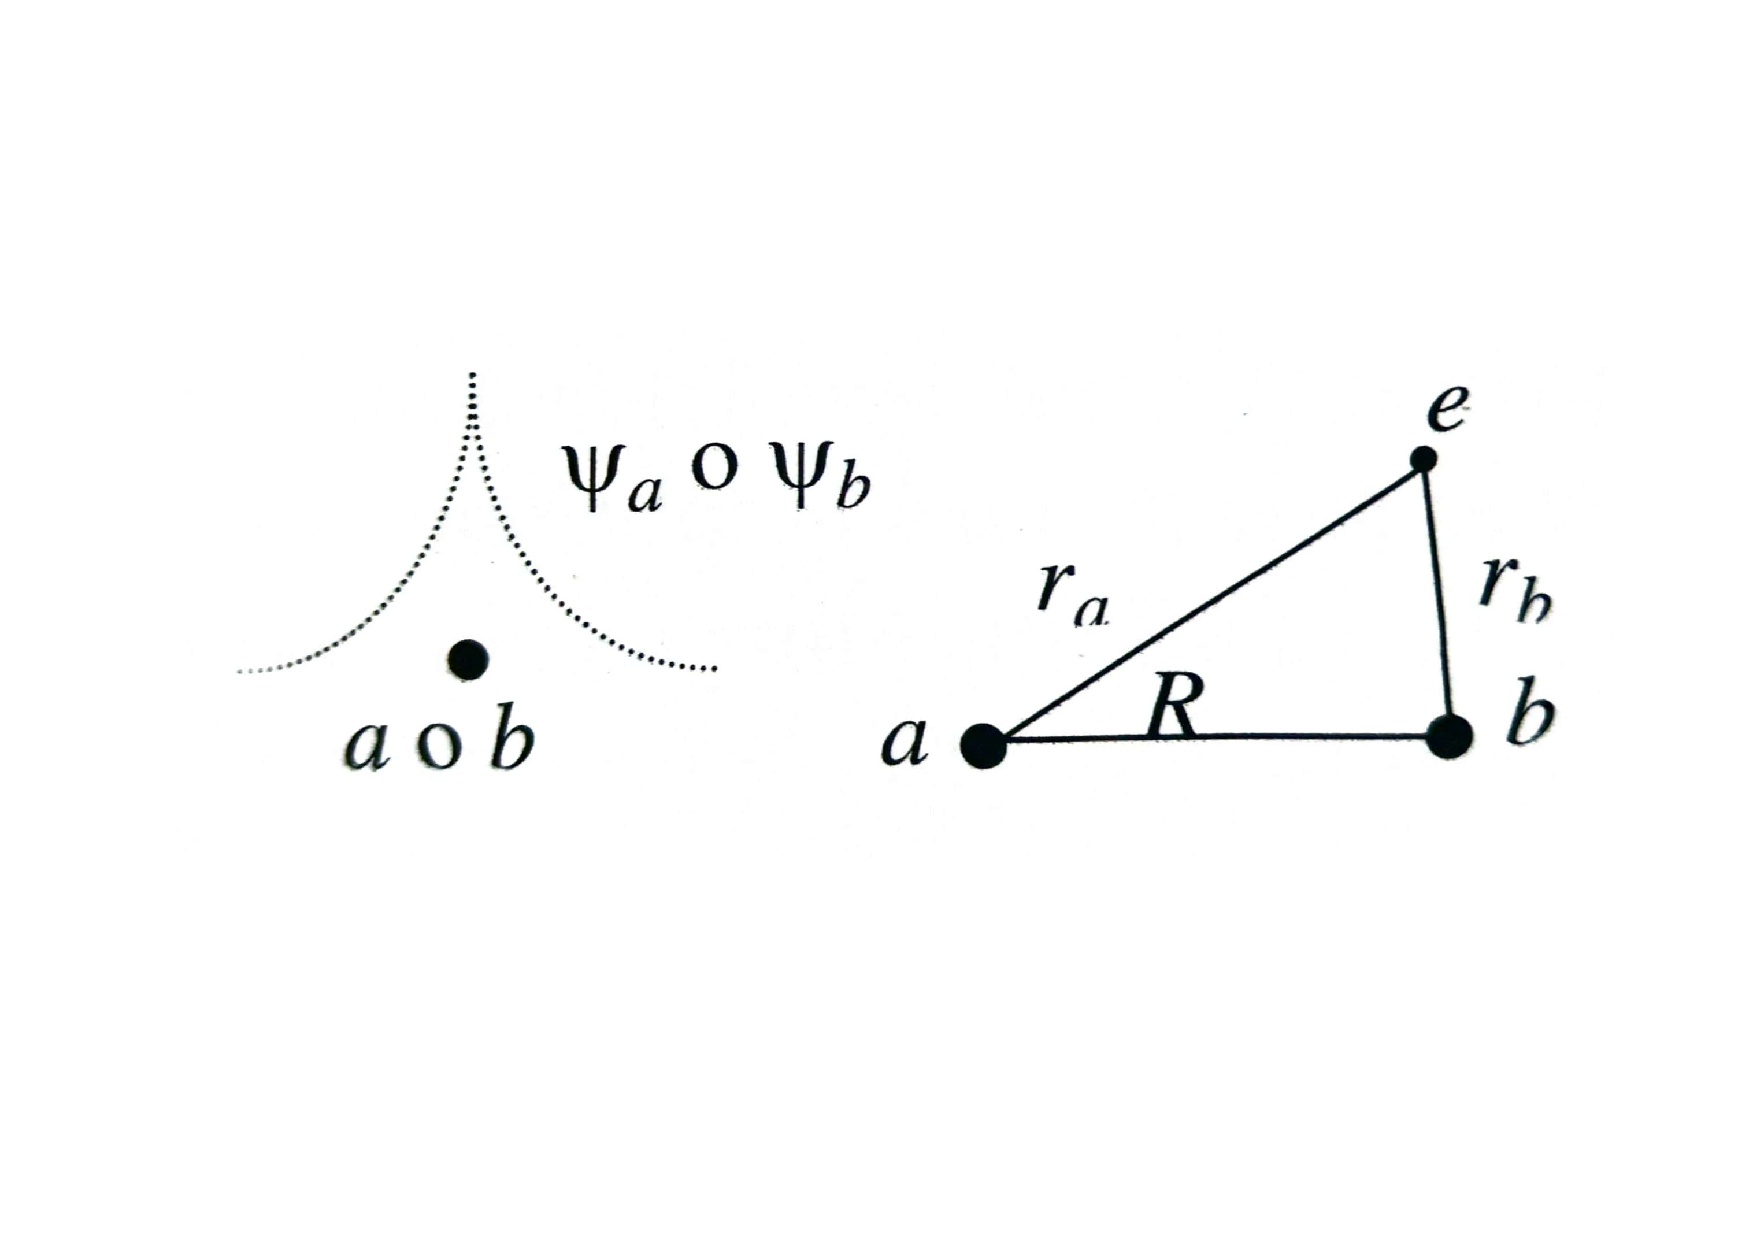
\includegraphics[scale=0.5]{Cuerpo/Ch_03/Fotos libro 3.pdf}
    \caption{Distribución de carga electrónica en torno al núcleo $a$ o al $b$ y posiciones relativas.}
    \label{Fig:03-04}
\end{figure}    


donde $C_a$ y $C_b$ son coeficientes a determinar. De la condición de normalización $\int_V \Psi \Psi^* \D^3 r = 1$ se obtiene 

\begin{equation}
    C_a^2 + 2 C_a C_b S + C_b^2 = 1 \quad \text{con} \quad S = \int_V \Psi_a^* \Psi_b \D^3 r \label{Ec:03-04-02}
\end{equation}

El valor medio de la energía se calcula según:

\begin{equation}
    \langle E \rangle = \int_V \Psi^* H \Psi \D^3 r = C_a^2 H_{11} + C_a C_b H_{12} + C_a C_b H_{21} + C_b^2 H_{22} \label{Ec:03-04-03}
\end{equation}
Los términos $H_{ij}$ vienen dados Por

\begin{align*}
    H_{11} = \int_V \Psi_a^* H \Psi_a \D^3 r = H_{22} = \int_V \Psi_b^* H \Psi_b \D^3 r = - E_0 + \frac{q^2}{R}-A \\
    H_{12} = \int_V \Psi_a^* H \Psi_b \D^3 r = H_{21} = \int_V \Psi_b^* H \Psi_a \D^3 r = - E_0 S + \frac{q^2}{R}S-J \\
\end{align*}
donde 

\begin{equation*}
    A = \int_V \Psi_a \frac{q^2}{r_b} \Psi_a \D^3 r  = \int_V \Psi_b \frac{q^2}{r_a} \Psi_b \D^3 r
\end{equation*}
es la llamada \textit{integral de Coulomb} [representa la interacción del protón \textit{a (b)} con el electrón alrededor del protón \textit{b(a)}] y

\begin{equation*}
    J = \int_V \Psi_a^* \frac{q^2}{r_b} \Psi_b \D^3 r = \int_V \Psi_b^* \frac{q^2}{r_b} \Psi_a \D^3 r > 0
\end{equation*}
es la \textit{integral de canje} (no tiene \textit{interpretación clásica}). En este caso, como la distribución de carga alrededor de ambos núcleos debe ser la misma

\begin{equation*}
    C_a^2 = C_b^2 \Rightarrow C_a = \pm C_b
\end{equation*}
con lo cual sustituyendo en la ecuación \ref{Ec:03-04-02} se obtiene que

\begin{align}
    C_a = C_b = \frac{1}{\sqrt{2(1+S)}} \Rightarrow \Psi_+ = \frac{\Psi_a+\Psi_b}{\sqrt{2(1+S)}} \\
    C_a = -  C_b = \frac{1}{\sqrt{2(1-S)}} \Rightarrow \Psi_- = \frac{\Psi_a-\Psi_b}{\sqrt{2(1-S)}} 
\end{align}
La solución que así resulta son dos nuevos autoestados, que se corresponden con las combinaciones simétrica y antisimétrica de $\Psi_a$ y $\Psi_b$, denominados orbital enlazante ($\Psi_+$) y orbital antienlazante ($\Psi_-$), de energías, respectivamente 

\begin{align}
\epsilon_+ = - E_0 + \frac{q^2}{R} - \frac{A+J}{1+S} \approx - E_0 -J \\
\epsilon_- = - E_0 + \frac{q^2}{R} - \frac{A-J}{1-S} \approx - E_0 +J
\end{align}
Como se ve en la figura \ref{Fig:03-05} la mayor densidad de carga es la solución simétrica en el espacio entre núcleos es la diferencia distintiva. Esta configuración es la de menor energía porque el electrón está menos confiando y tiene por tanto una menor energía cinética $E_c$ (valor medio de $\nabla^2 \Psi$ menor). Lo mismo vale para la energía potencial $E_p$ por cuanto el electrón, en el estado simétrico, está en medio más cerca de ambos núcleos a la vez.


La energía de disociación (energía de cohesión), $E_D$, y la distancia internuclear en el equilibrio , $R$, de la molécula H$_2^+$, son respectivamente 2.79 eV y 1.06  \unit{\angstrom}. Evaluando las integrales $H_{ij}, \ A, \ S$, etc. precedentes, y utilizando funciones de onda $1s$ para los orbitales atómicos ($\Psi \propto e^{-r/a_0}$ donde $a_0=0.529\unit{\angstrom}$ es el \textit{radio de Bohr}). Si además de orbitales $1s$ se incluyen los orbitales $2s$ y $2p$ en la ecuación \ref{Ec:03-04-01} se obtiene $E_D = 2.71 \unit{\eV} $ y $R=1.06 \unit{\angstrom}$ de modo que el modelo da cuenta cuantitativamente de la molécula H$_2^+$.


\begin{figure}[h!] \centering
    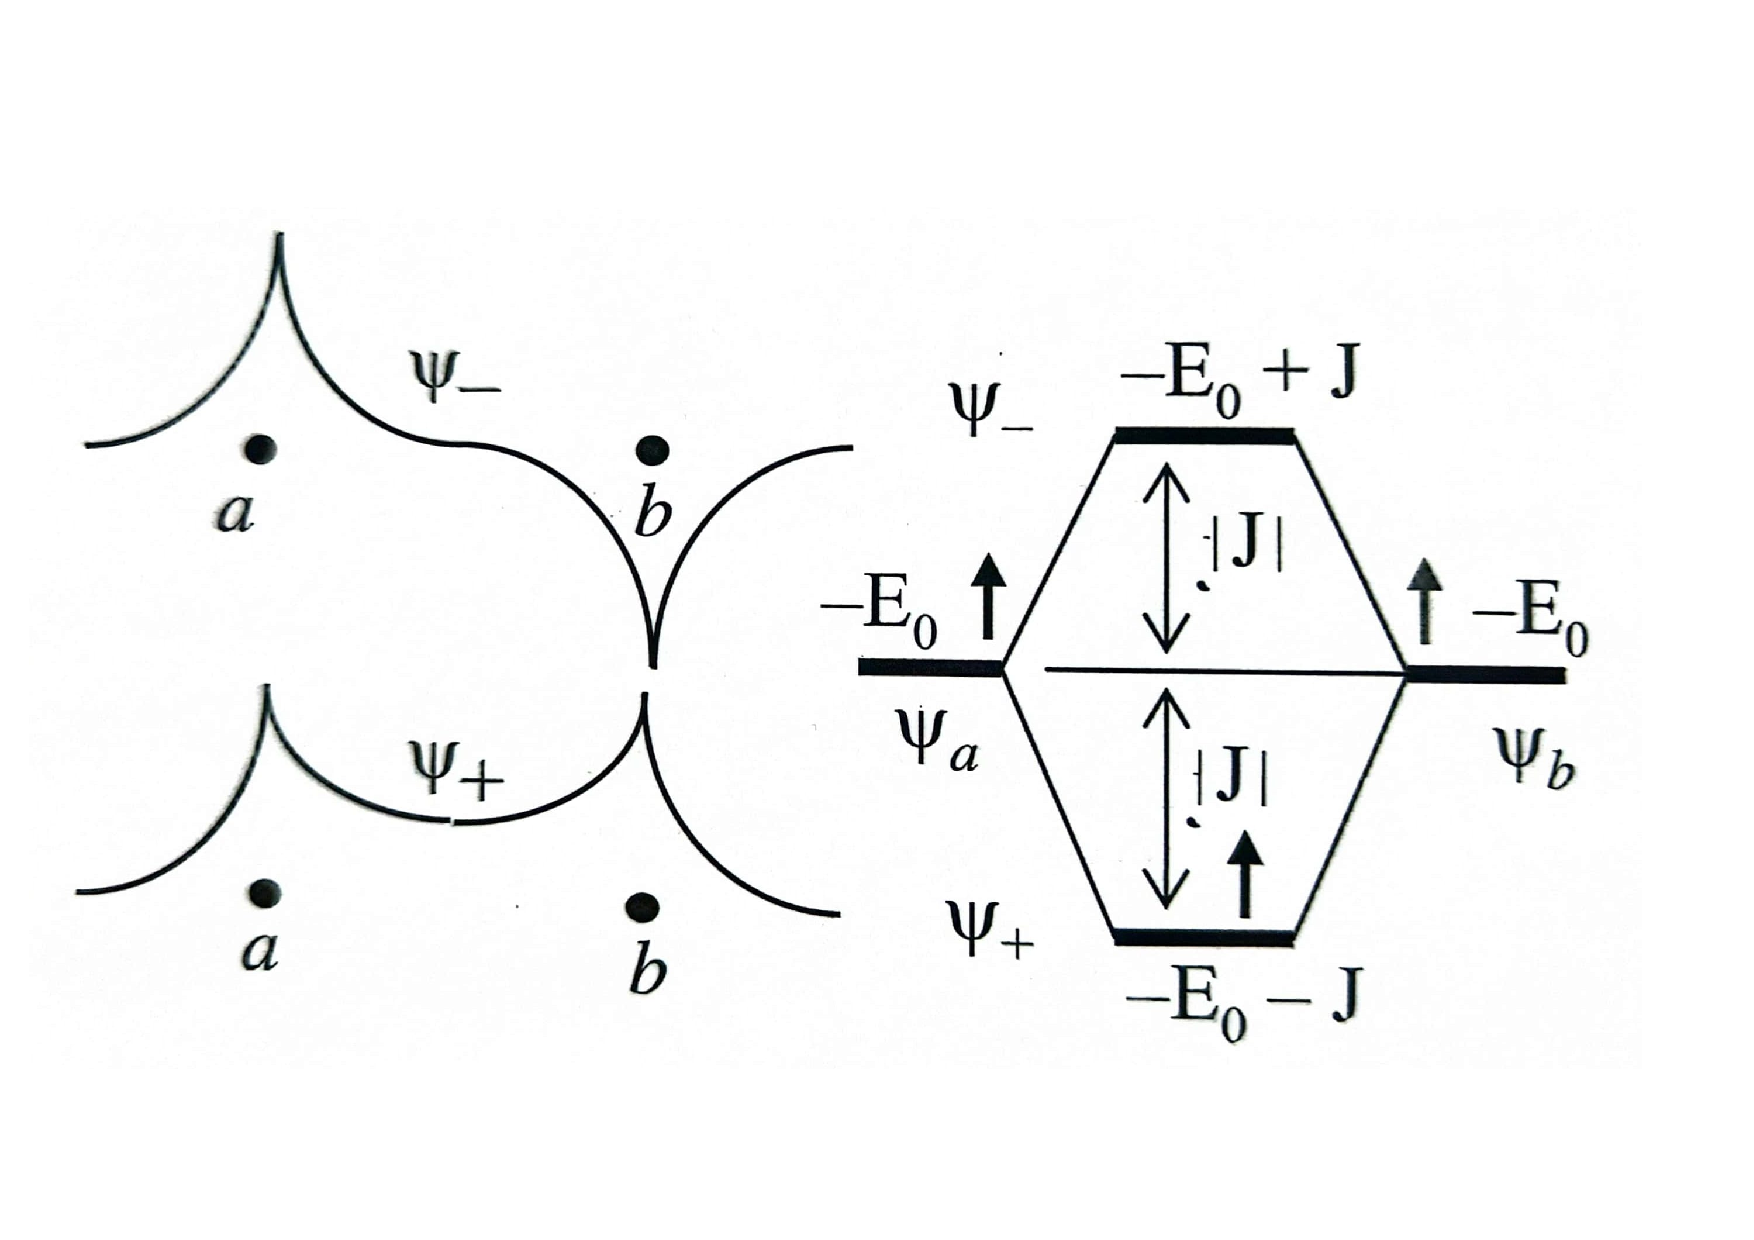
\includegraphics[scale=0.5]{Cuerpo/Ch_03/Fotos libro 4.pdf}
    \caption{Distribución de carga electrónica para las soluciones $\Psi_-$ y $\Psi_+$ y los correspondientes niveles de energía.}
    \label{Fig:03-05}
\end{figure}    



\subsection{La molécula de hidrógeno (H$_2)$}

Es el ejemplo más sencillo de molécula neutra y prototipo de enlace covalente: enlace entre átomos (\textit{objetos} neutros) por medio de electrones igualmente compartidos. Este mecanismo necesariamente comprende el tomar un electrón de cada uno de ellos para formar el enlace. El hamiltoniano es ahora

\begin{equation*}
    H = - \frac{\hbar^2}{2m} (\Delta_1 + \Delta_2) - \frac{q^2}{r_{a_1}} - \frac{q^2}{r_{a_2}} - \frac{q^2}{r_{b_1}} - \frac{q^2}{r_{b_1}} + \frac{q^2}{r_{12}} - \frac{q^2}{R}
\end{equation*}
La presencia del término $q^2/r_{12}$, qeu da cuenta de la interacción repulsiva entre los dos elecrrones, impide obtener una solución exacta para la molécula de hidrógeno. Ignorando este término, en la llamada \textit{aproximación de electrones independientes}, pueden aplicarse directamente los resultados obtenidos para el ion H$_2^+$: la existencia de un estado enlazante y otro antienlazante. El estado de más baja energía se obtiene poniendo ambos electrones en el orbital enlazante, con sus espines opuestos para no violar el principio de exclusión, como se indica en la figura . Este hecho está de acuerdo con el llamado \textit{principio de máximo solapamiento}, según la cual la configuración más estable es aquella en la que las funciones de onda electrónicas individuales solapan lo máximo posible (el aumento de la energía de interacción electroestática se compensa con la disminución de la energía de confinamiento). Este principio exige que, en general, un átomo no puede formar más enlaces covalentes que electrones tenga fuera de capas cerradas (en particular, el H sólo puede formar un enlace). Por esto se dice que el enlace covalente es \textit{saturable}. 

\begin{figure}[h!] \centering
    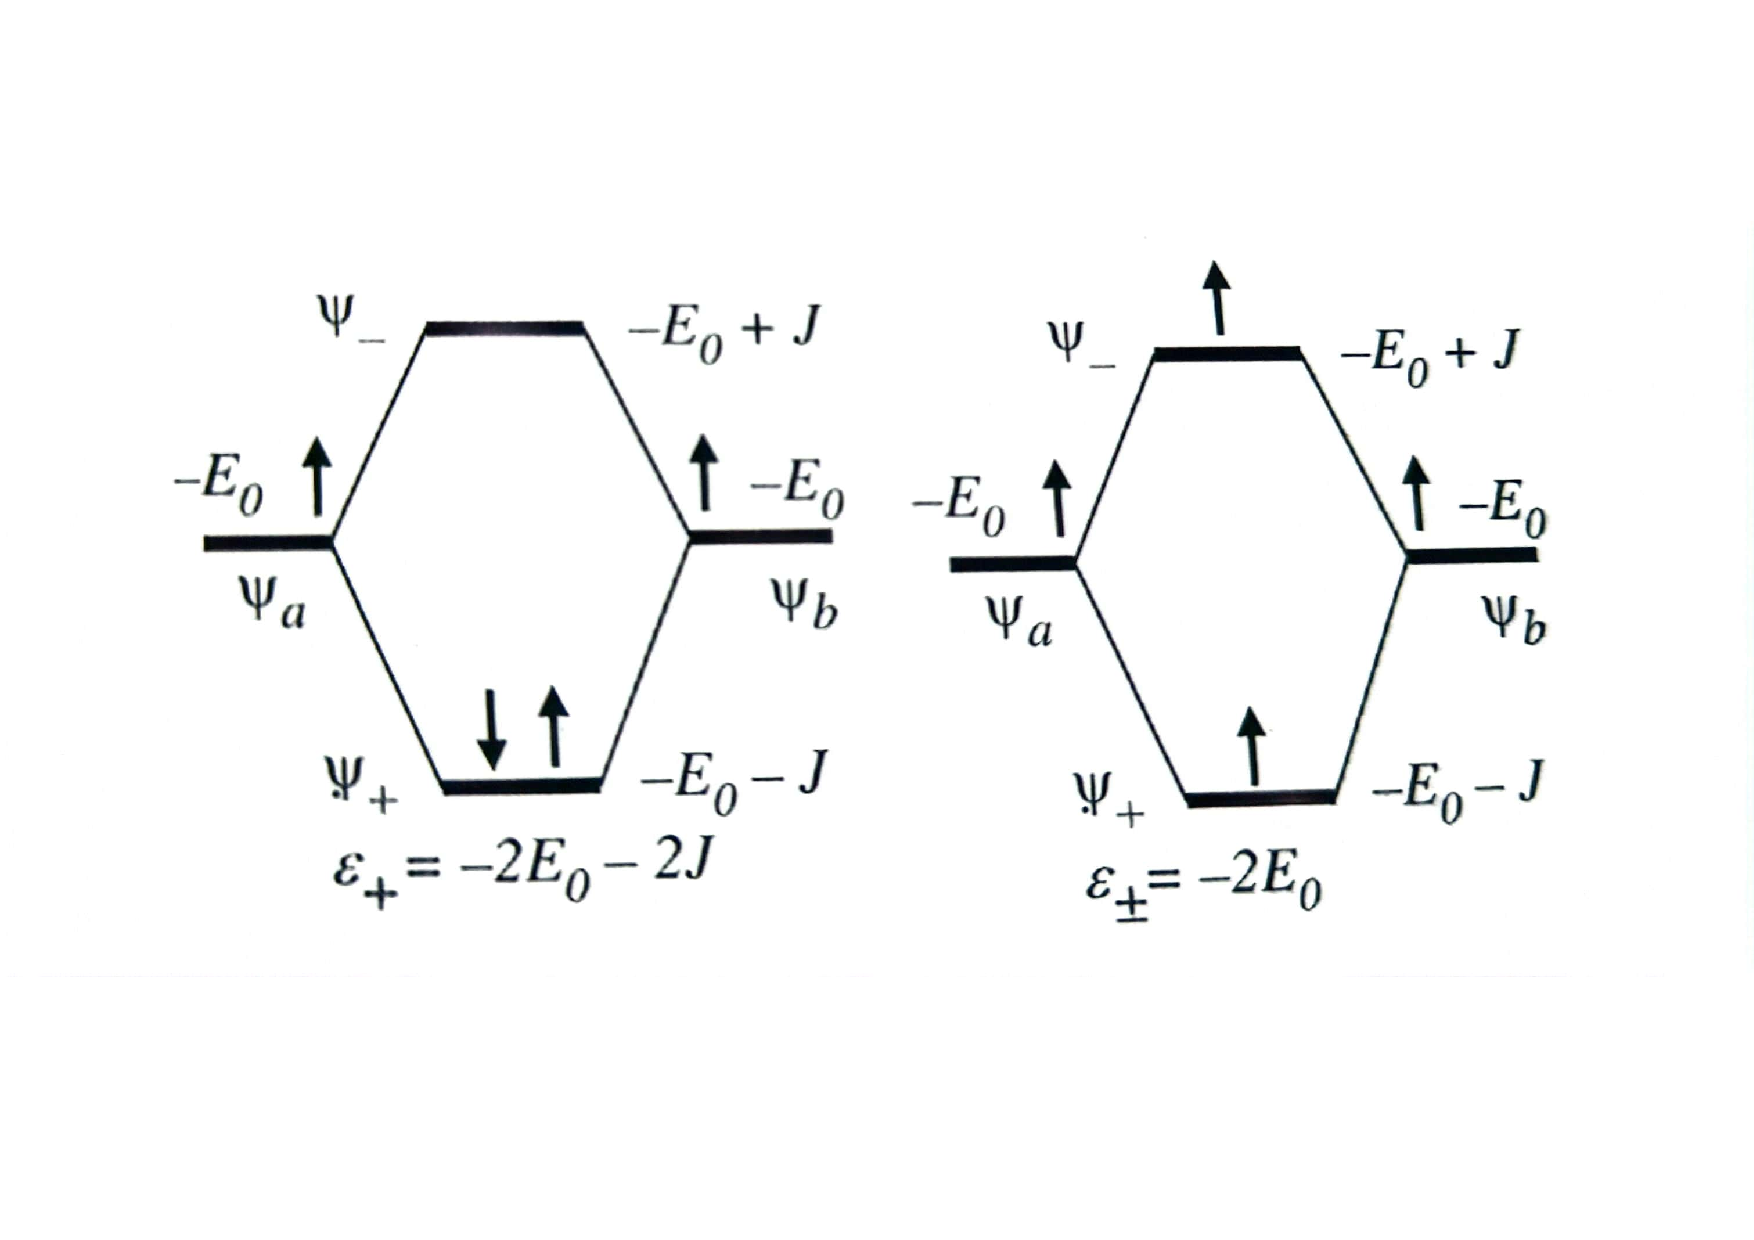
\includegraphics[scale=0.5]{Cuerpo/Ch_03/Fotos libro 5.pdf}
    \caption{Energía con dos electrones en el estado enlazante (espines opuestos) y con un electrón en el estado enlazante.}
    \label{Fig:03-06}
\end{figure}    


Para obtener la energía de cohesión de la molécula H$_2$ existen dos métodos aproximados que se aplican en general a otras moléculas y sólidos: el de \textit{orbitales moleculares} y el de \textit{electrones de valencia}. En el primero el estado molecular fundamental se representa por la función 

\begin{equation}
    \Psi (\rn_1, \rn_2) = \Psi_+ (\rn_1) \Psi+ (\rn_2)
\end{equation}
que es simétrica bajo el intercambio de las coordenadas electrónicas (para hacer la función de onda \textit{total} antisimétrica, laf unción de onda de espín debe ser antisimétrica $\Rightarrow$ espines antiparalelos) y para $\Psi_+$ se utiliza el orbital enlazante obtenido para el ion H$_2^+$, $\Psi_+ \propto \Psi_a + \Psi_b$. Así:

\begin{equation}
    \Psi (\rn_1, \rn_2) = \ccorchetes{\Psi_a (\rn_1)+\Psi_b (\rn_1)}\ccorchetes{\Psi_a(\rn_2)+\Psi_b(\rn_2)} \label{Ec:03-04-08}
\end{equation}
En la aproximación de elctrones independientes y utilizando orbitales $1s$ para las funciones atómicas $\Psi_a$ y $\Psi_b$ se obtiene $E_D = 2.65 \unit{\eV}$ y $R=1.6a_0$, a comparar con los experimentales $E_D = 4.72 \unit{\eV}$ y $R=1.40a_0$. El origen de este desacuerdo se halla en el error cometido por la necesiddad de tener en cuenta otros orbitales además del $1s$, pero sobre todo por aproximar la función de onda $\Psi(r_1,r_2)$ según la ecuación \ref{Ec:03-04-08}. Si se desarrolla el producto de esta ecuación se obtiene 

\begin{equation}
    \Psi (\rn_1 , \rn_2) = \Psi_a (\rn_1) \Psi_a (\rn_2) + \Psi_b (\rn_1) \Psi_b (\rn_2) + \Psi_a (\rn_1) \Psi_b (\rn_2) + \Psi_a (\rn_2) \Psi_b (\rn_1) \label{Ec:03-04-10}
\end{equation}
Como $\Psi_a$ es grande cerca del núcleo, $a$ y $\Psi_b$ lo cerca del núcleo $b$, los dos primero sumandos de la ecuación \ref{Ec:03-04-10} tienen una interpretación física muy diferente de la de los dos últimos. Éstos dan la amplitud de probabilidad de encontrar dos átomos neutros de hidrógeno (H+H), mientras que los dos primeros sumandos dan la amplitud de probabilidad de encontrar un protón \textit{desnudo} H$^+$ y un ion hidrógeno negativo H$^+$ y un ion hidrógeno negativo H$^-$ (H$^+$+H$^-$). En la aproximación de electrones independientes estos estados tienen la misma energía (un electrón tiene una energía de enlace de 13.6 eV con un protón independientemente de si ya está enlazado con otro electrón) y por ello sus funciones de onda se mezclan con igual peso. Sin embargo, es bien conocido que un electrón se enlaza con un átomo neutro de hidrógeno para formar H$^-$ sólo por 0.7 eV (debido a la fuerza de repulsión del primer electrón). Por lo tanto, al menos a separaciones a las que se pueda diferenciar claramente entre los estados H$^+$+H$^-$ y H+H, la aproximación de electrones independientes es mala. Existen refinamientos dentro del método de \textit{orbitales moleculares} que mejoran el acuerdo con los datos experimentales, en particular, dando \textit{pesos} distintos a los sumandos de la ecuación \ref{Ec:03-04-10}.  

El método de \textit{electrones de valencia} desprecia por completo la configuración  H$^+$+H$^-$, de modo que usa la función de onda aproximada

\begin{equation}
    \Psi (r_1,r_2) =  \Psi_a (\rn_1) \Psi_b (\rn_2) + \Psi_a (\rn_2) \Psi_b (\rn_1)
\end{equation}
Utilizando el hamiltoniano completo (sin despreciar el término repulsivo), orbitales $1s$ para $\Psi_a$ y $\Psi_b$, y aplicando el cálculo variacional se obtiene $E_D = 3.14$ eV y $R=1.64a_0$ que está más cerca de los valores experimentales. El acuerdo se mejora consdierando además orbitales $p$, la polarización de los orbitales atómicos.

\subsection{Hibridación}

La hibridación es una característica del enlace covalente que se origina en átomos con varios electrones fuera de una capa cerrada. De acuerdo con el principio genérico de \textit{máximo solapamiento} que rige el enlace covalente entre orbitales $1s$ del H$_2$ ($1s^2$) es más débil que el enalce entre orbitales $2p$ del F$_2$ ($1s^22s^22p_x^22p_y^22p_z^1$), por ser esta más direccional (\textit{lóbulos p}) y por tanto permitir más solapamiento. En medio de ambos está el de la molécula HF formado por el solapamiento del orbital $1s$ del hidrógeno y el $2p$ del flúor.

Para estar en condiciones de máximo solapamiento puede ser rentable que se produzca primero una \textit{promoción} (excitación) electrónica dando lugar a la fomración de nuevos estados, los llamados \textit{orbitales híbridos}, que serán los que se enlacen con orbitales híbridos de átomos vecinos recuperando en el enlace la energía invertida en la promoción. Por ejemplo, en la formación de la molécula Cl$_2$Be (Be: $1s^22s^2$, Cl: $1s^22s^22p^63p_x^13p_y^23p_z^2$) previamente en el Be se produce la promoción $1s^2 2s^2 \rightarrow 1s^2 2s^1 2p_x^1$ formandose luego los llamados híbridos $sp$, como se ilustra en la figura \ref{Fig:03-07} (izquierda), cada uno de los cuales se enlazaccon el orbital $3p_x$ de cada átomo de cloro.

\begin{figure}[h!] \centering
    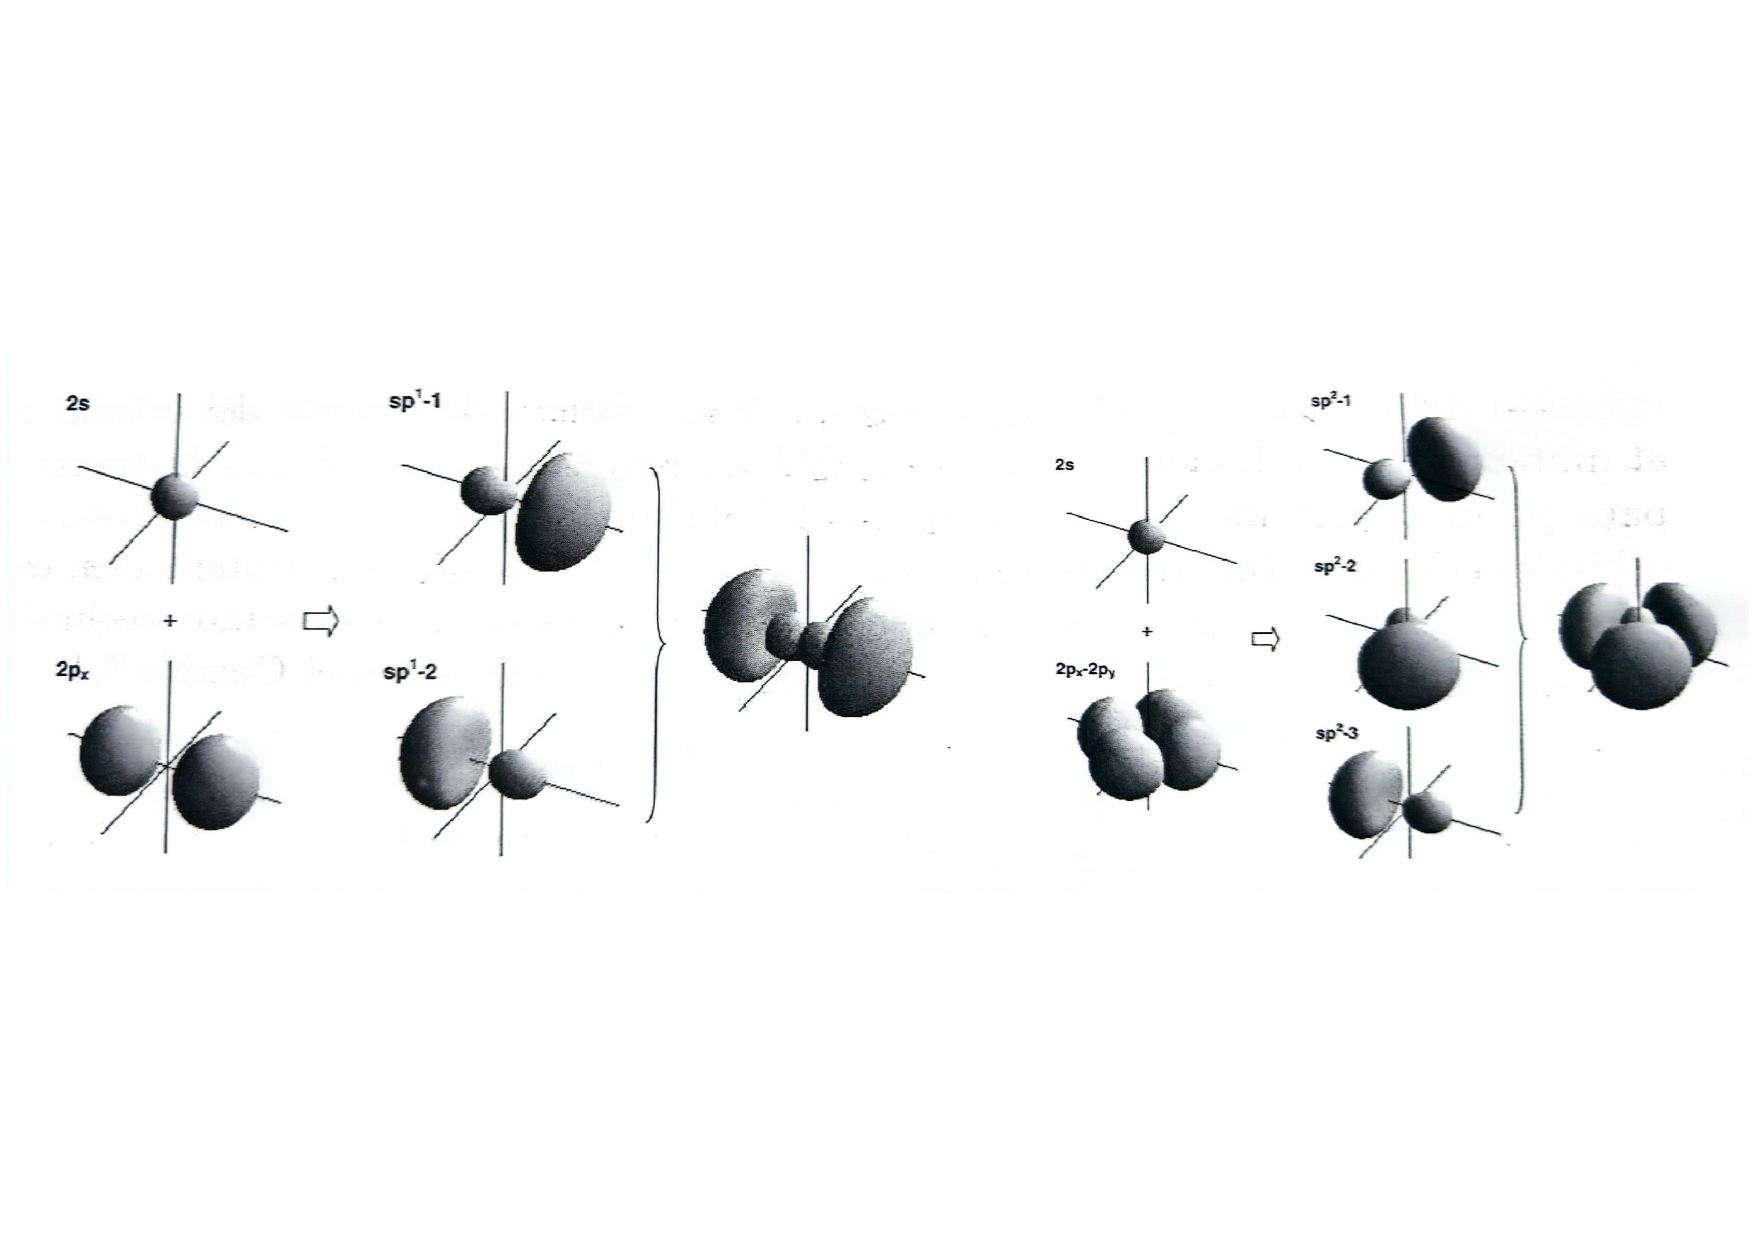
\includegraphics[scale=0.5]{Cuerpo/Ch_03/Fotos libro 6.pdf}
    \caption{Formación de los orbitales híbridos $sp^1$ (izquierda) y $sp^2$ (derecha).}
    \label{Fig:03-07}
\end{figure}    

\begin{figure}[h!] \centering
    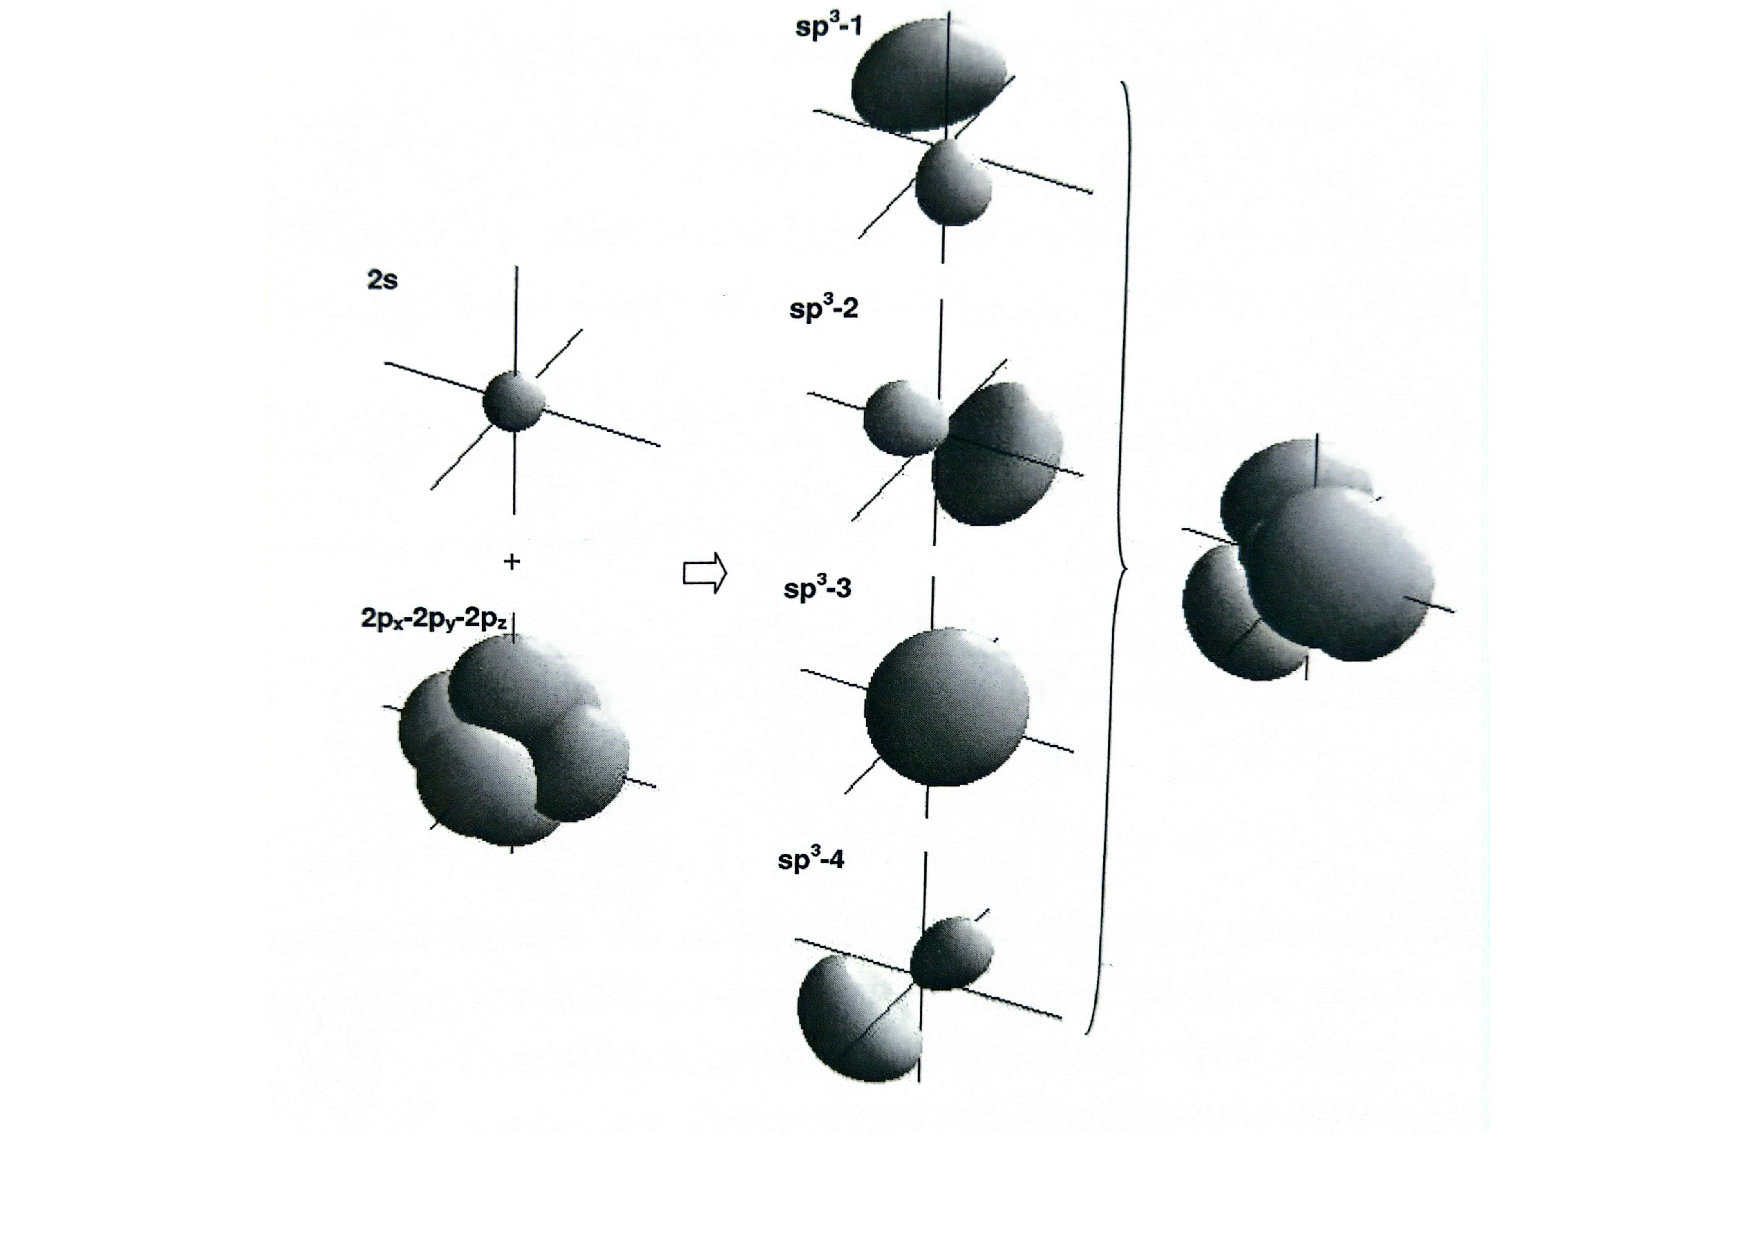
\includegraphics[scale=0.5]{Cuerpo/Ch_03/Fotos libro 7.pdf}
    \caption{Orbitales híbridos $sp^3$.}
    \label{Fig:03-08}
\end{figure}    


La molécula BH$_3$ resulta de la promoción $1s^22s^22p_x^1\rightarrow 1s^2 2s^1 2p_x^12p_y^1$ del boro dando lugar a los híbridos $sp_2$, como se muestra en la figura \ref{Fig:03-07} (derecha) con cada uno de los cuales se enlaza a un H. 

Otro ejemplo son los híbridos $sp^3$ tetraédricos del C que resultan de la promoción previa $1s^22s^22p_x^12p_y^1 \rightarrow 1s^22s^12p_x^12p_y^12p_z^1$. Se forman luego, por combinación lineal de los estados, orbitales híbricos que apuntan a los vértices de un tetaedro regular (figuras \ref{Fig:03-08} y \ref{Fig:03-09} (a)) y constituyen la base del cristal de diamante y de los semiconductores. 

Los enlaces se forman por el acoplamiento de orbitales híbridos de dos átomos vecinos $a,b$ que apunten en la misma dirección 

\begin{equation}
    \Psi = C_a |h(a) \rangle + C_b |h(b) \rangle
\end{equation}
El tratamiento es análogo al que se sigue para la molécula H$_2$ (los orbitales híbridos $h$ son sólo algo más complejos que los atómicos al igual que el hamiltoniano) y se obtienen también dos soluciones: un estado enlazante y otro antienlazante. En el estado fundamental los electrones ocuparán los estados de más baja energía (estado enlazante), como se indica en la figura \ref{Fig:03-09}(b).

En la aproximación del \textit{orbital enlazante}, el cristal puede verse como una estructura periódica de orbitales enlazantes entre los átomos vecinos. La energía de cohesión del cristal es $\frac{z}{2} N E_{1\text{enlazante}}$ siendo $N$ el número de átomos del cristal, $z$ el número de coordinación, $E_{1\text{enlazante}} = 2 (E_+ - E_0  - E_{\text{prom}})$ y $E_{\text{prom}}$ la energía para promocionar un electrón a un orbital de un nivel superior y así producir orbitales híbridos. Incluyendo los llamados \textit{efectos de metalicidad} (interacción de un orbital enlazante de un átomo con los antienlazantes de los átomos vecinos), esta aproximación de las energías de la tabla \ref{Tab:03-04}.


\begin{table}[h!]  \centering
\begin{tabular}{c|cccc}
 & C & Si & Ge & Sn  \\ \hline
 Calculada & 14.2 & 5.0 & 4.6 & 3.5 \\
 Experimental & \textbf{7.3} & \textbf{4.6}&  \textbf{3.9} &  \textbf{3.1}
\end{tabular}
\caption{Energías de cohesión (eV/átomo) de algunos cristales covalentes.}
\label{Tab:03-04}
\end{table}

\begin{figure}[h!] \centering
    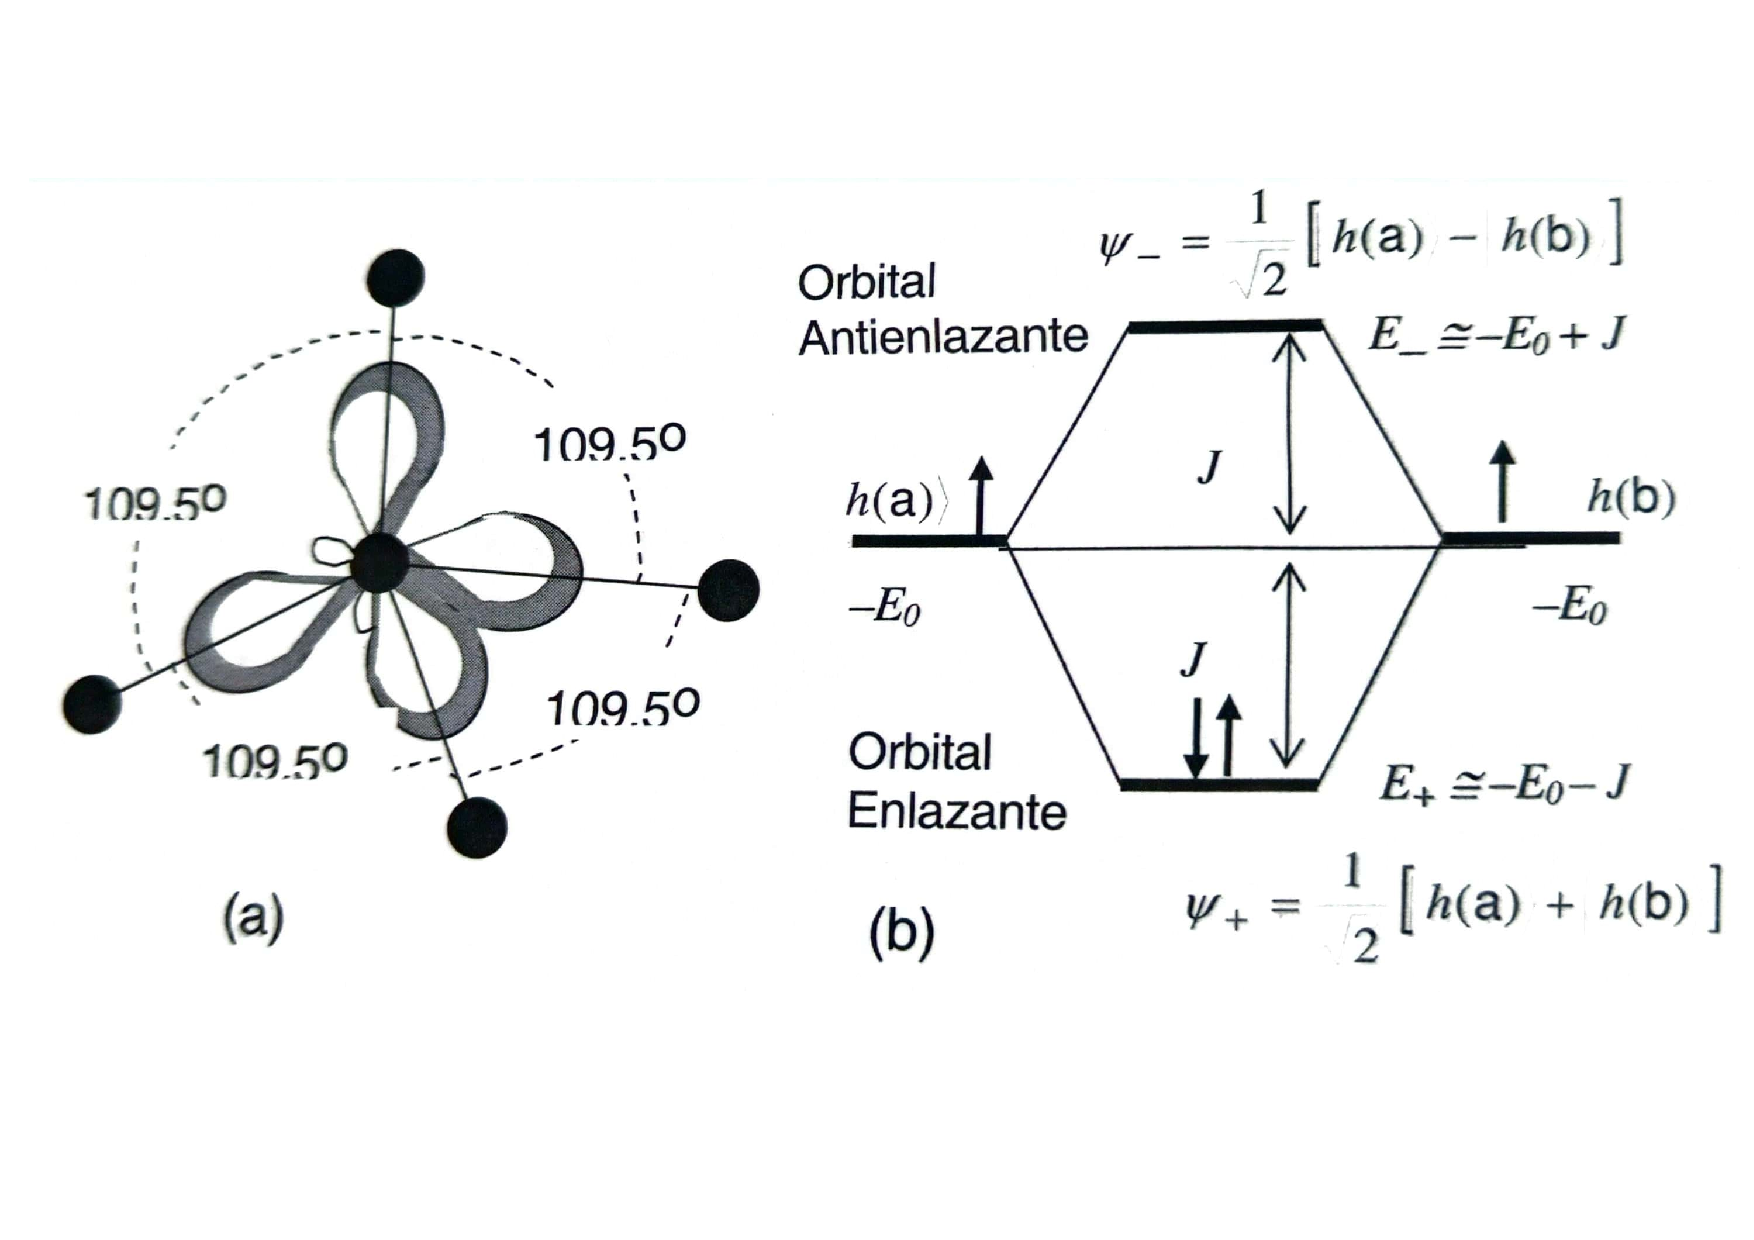
\includegraphics[scale=0.5]{Cuerpo/Ch_03/Fotos libro 8.pdf}
    \caption{Niveles de energía asociados al enlace entre orbitales híbridos.}
    \label{Fig:03-09}
\end{figure}    

\section{Cristales metálicos}

El enlace metálico puede considerase como caso límite del enlace iónico, en el cual los iones negativos son precisamente electrones. La diferencia crítica es que la masa muy pequeña del electrón hace que su energía del punto cero sea grande, de modo que no está localizado en un punto de red, lo que a su vez da cuenta de la alta conductividad eléctrica. 

Considérese el modelo idealizado (figura \ref{Fig:03-10}) consistente en iones positivos puntuales de valencia $Z$ situados regularmente y bañados por un mar de carga negativa que consideremos confinada en volúmentes esféricos de radio $R$ alrededor de cada ion, de modo que la carga electrónica neta alrededor de cada ion es $Ze(\Rightarrow$ densidad de carga $n=Ze/\frac{4}{3}\pi R^3$). $R$ o equivalentemente la concentración $n$ es desconocida y será determinada por la condición de energía mínima. 


\begin{figure}[h!] \centering
    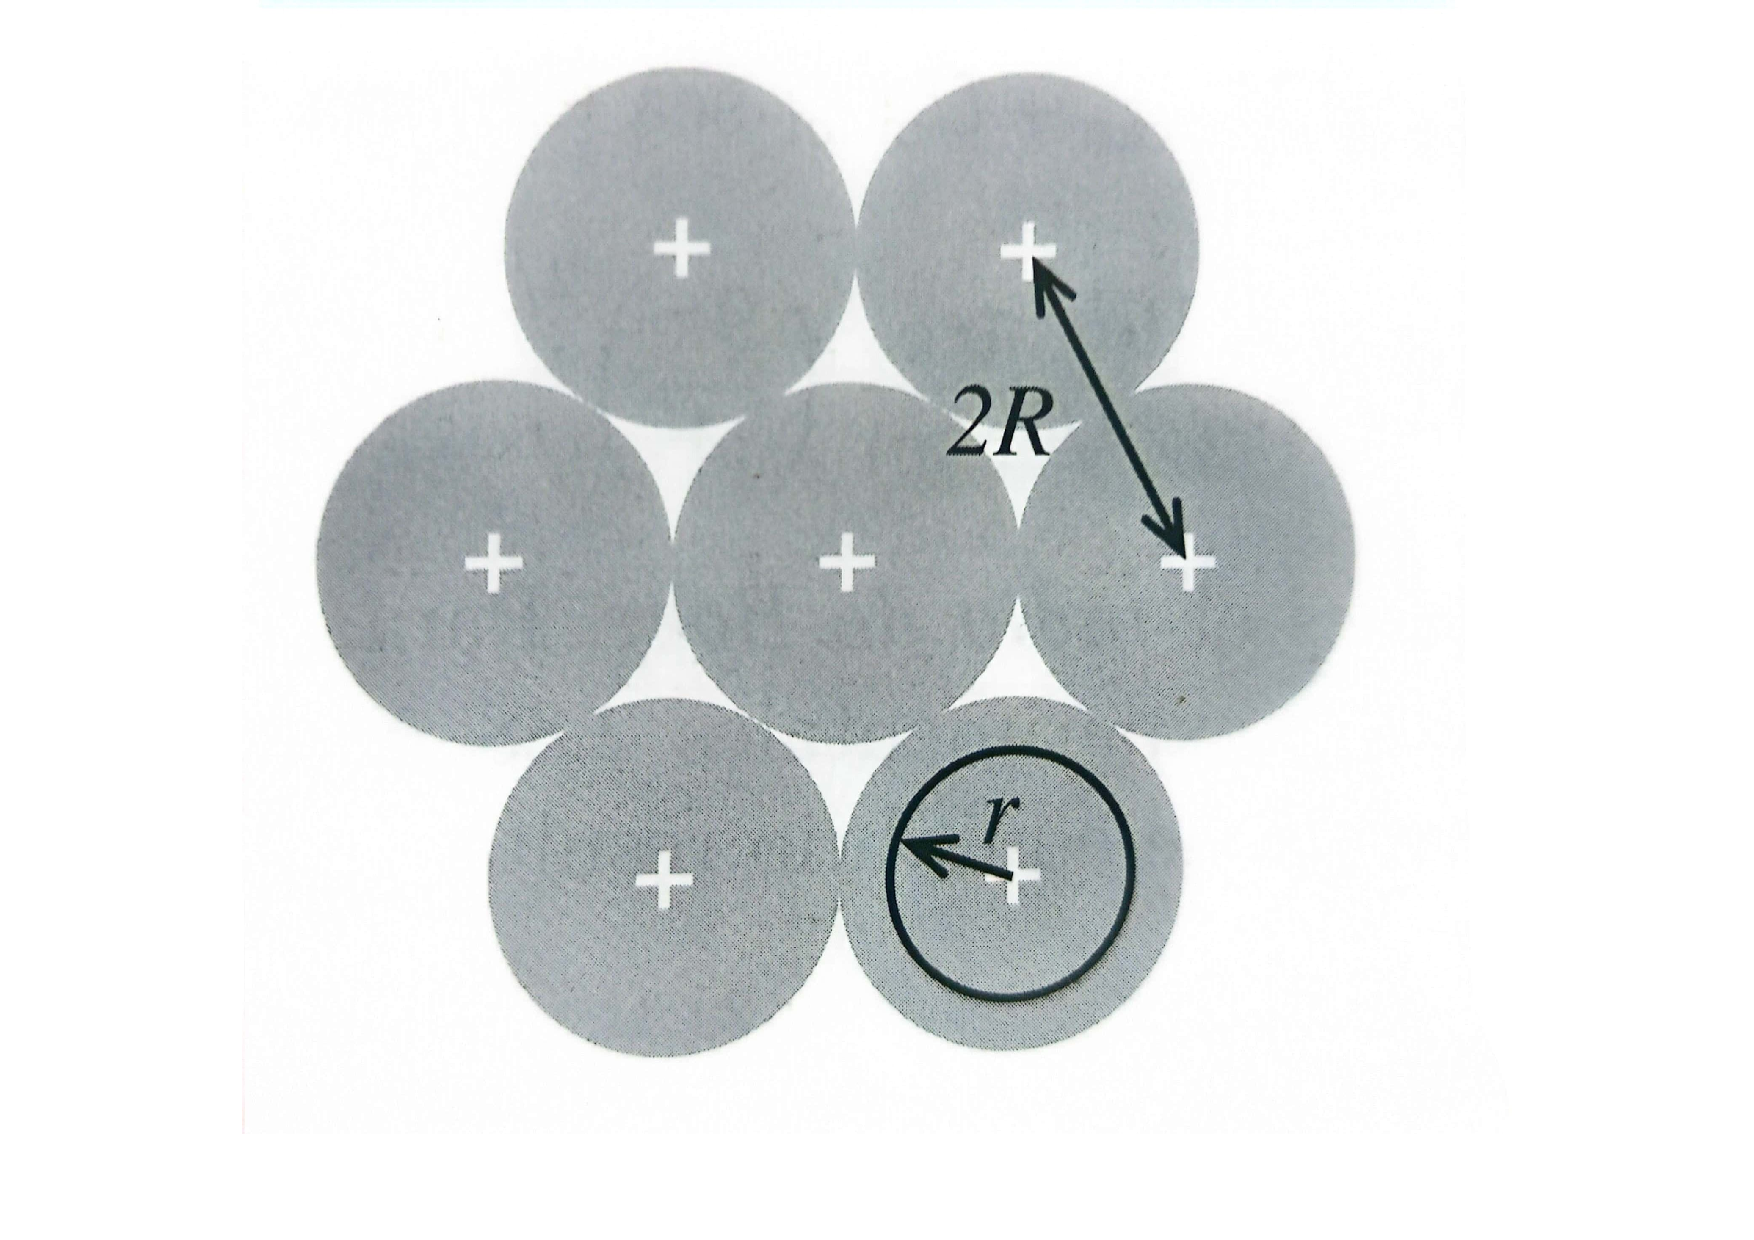
\includegraphics[scale=0.5]{Cuerpo/Ch_03/Fotos libro 9.pdf}
    \caption{Modelo de cirstal metálico.}
    \label{Fig:03-10}
\end{figure}    


Para determinar la energía comenzamos por calcular la energía potencial. La carga a distancia $r$ de un ion es

\begin{equation}
    q(r) = Ze - n \frac{4}{3} \pi r^3 = Ze \parentesis{1-\frac{r ^3}{R^3}}
\end{equation}
y entonces el potencial electroestático es $\phi(r) = q(r)/4\pi \epsilon_0 r$. La energía electroestática atractiva ion-electrón será $\D U_{\text{atrac}} = \phi \D q$, es decir,

\begin{equation}
    \D U_{\text{atrac}} = \underbrace{\frac{Ze}{4 \pi \epsilon_0 r} \parentesis{1-\frac{r^3}{R^3}}}_{\phi} \underbrace{\frac{-3Ze}{R^3}r^2 \D r}_{\D q} = -3Z^2 e^2 \parentesis{1-\frac{r^3}{R^3}} \frac{r\D r}{4 \pi \epsilon_0 R^3}
\end{equation}
Integrando sobre el volumen en $R$ se obtiene la energía potencial por átomo

\begin{equation}
    U_{\text{atrac}} = \frac{-3Z^2e^2}{4 \pi \epsilon_0 R^3} \int_0^R \parentesis{1-\frac{r^3}{R^3}} r \D r = - \frac{9Z^2 e^2}{40 \pi \epsilon_0 R}
\end{equation}
Esta energía potencial contabiliza la interacción atractiva entre iones y electrones así como la repulsión electrón-electrón. Obsérvese que en este modelo no hay interacción entre átomos por ser éstos neutros y esféricamente simétricos. 

Falta la energía cinética de los electrones. Esta es muy elevada debido fundamentalmente a su carácter fermiónico: el \textit{principio de exclusión de Pauli} los obliga a ocupar estados distintos, cada vez más energéticos, de modo que incluso a $T=0$K los más energéticos alcanzan una energía cinética del orden de $\sim$eV. Como se verá en el capítulo \ref{Ch:06}, la energía cinética total de un gas de electrones de concentración numérica $n$ viene dada Por

\begin{equation}
    U_{\text{cinet}} = \frac{3\hbar^2 (3 \pi^2 n^{2/3})}{10m}
\end{equation}
donde $m$ es la masa del electrón. Como $n=Ze/\frac{4}{3}\pi R^3$, se tiene que 

\begin{equation}
    U_{\text{cinet}} = \frac{3\hbar^2 (9 \pi \frac{Z}{r})}{10mR^2}
\end{equation}
Así como la energía potencial aumenta (se hace menos negativa) al aumentar R, por cercanía de cargas opuestas la energía cinética disminuye porque el confinamiento electrónico es menor. En el equilibrio (radio $R_0$, interdistancia $2R_0$), se debe cumplir que $U_{\text{tot}}=U_{\text{atrac}}+U_{\text{cinet}}$ sea mínima. Imponiendo esta condición resulta 

\begin{equation}
    2R_0 = \frac{16\hbar^2 \pi \epsilon_0}{3Z^{4/3} e^2 m}\parentesis{\frac{9\pi}{4}}^{2/3} = \frac{4.9}{Z^{4/3}} a_0
\end{equation}
donde $a_0 = \hbar^2 4 \pi \epsilon_0 / e^2 m$ es el \textit{radio de Bohr}. Para $Z=1$ se tiene $2R_0 \approx 2.6 \unit{\angstrom}$ a comparar con los valores experimentales $2.88 \unit{\angstrom}$ del Au y $2.56 \unit{\angstrom}$ del Cu, por ejemplo. A su vez la energía de equilibrio resultante

\begin{equation}    
    U_{\text{tot}} (R_0) = - \frac{9e^2}{80 \pi \epsilon_0 R_0} \approx -5\unit{-\eV / at}
\end{equation}
a comparar con $-3.81 \unit{-\eV / at}$ del Au o $-3.49\unit{-\eV / at}$ del Cu. 

Aunque este modelo recoge lo esencial del enlace metálico, es limitado en cuanto que es independiente de la estructura o no tiene en cuenta otros electrones que los de valencia. Por ello, no puede explicar, por ejemplo, por qué algunos metales cristalizan en el sistema \textit{hcp} y otros lo hacen en el \textit{bcc} o \textit{fcc} o por qué la energía de enlace en el W es tan alta como 8.9 \unit{\eV / at}.

% Graficar el potencial de lenard jones